\chapter{Билет №12}

\section*{Создание виртуальных файловых систем. Структура, описывающая файловую систему. Регистрация и дерегистрация файловой системе. Монтирование файловой системы. Точка монтирования. Кэширование в системе. Кэши SLAB, функции для работы с кэшем SLAB. Примеры из лабораторной работы. Функции, определенные на файлах (struct file\_operations), функции, определенные на файлах, и их регистрация. Пример из лабораторной работы по файловой системе /proc.}

\section{Файловая подсистема}
Файл --- важнейшее понятие в файловой подсистеме. Файл --- информация, хранимая во вторичной памяти или во вспомогательном ЗУ с целью ее сохранения после завершения отдельного задания или преодоления ограничений, связанных в объемом основного ЗУ.

Файл --- поименованная совокупность данных, хранимая во вторичной памяти (возможно даже целая). Файл --- каждая индивидуально идентифицированная единица информации.

Существует 2 ипостаси файла:
\begin{enumerate}
	\item файл, который лежит на диске;
	\item открытый файл (с которым работает процесс).
\end{enumerate}

Открытый файл --- файл, который открывает процесс.

Файл != место на диске. В мире современной вычислительной техники файлы имеют настолько большие размеры, что не могут храниться в непрерывном физическом адресном пространстве, они хранятся вразброс (несвязанное распределение).

Файл может занимать разные блоки/сектора/дорожки на диске аналогично тому, как память поделена на страницы. В любой фрейм может быть загружена новая страница, как и файл. 

Также, важно понимать адресацию. 

Соответственно, система должна обеспечить адресацию каждого такого участка.

\begin{quote}
	ОС является загружаемой программой, её не называют файлом, но когда компьютер включается, ОС находится во вторичной памяти. Затем с помощью нескольких команд, которые находятся в ПЗУ, ОС (программа) загружается в ОЗУ. При этом выполняется огромное количество действий, связанных с управлением памятью, и без ФС это сделать невозможно. Любая ОС без ФС не может быть полноценной.
\end{quote}

Задача ФС --- обеспечивать сохранение данных и доступ к сохраненным данным (обеспечивать работу с файлами).

Чтобы обеспечить хранение файла и последующий доступ к нему, файл должен быть изолирован, то есть занимать некоторое адресное пространство, и это адресное пространство должно быть защищено. Доступ обеспечивается по тому, как файл идентифицируется в системе (доступ осуществляется по его имени).

ФС --- порядок, определяющий способ организации хранения, именования и доступа к данным на вторичных носителях информации.

\begin{quote}
	File management (управление файлами) --- программные процессы, связанные с общим управлением файлами, то есть с размещением во вторичной памяти, контролем доступа к файлам, записью резервных копий, ведением справочников (directory).
	
	Основные функции управления файлами обычно возлагаются на ОС, а дополнительные --- на системы управления файлами.
	
	Доступ к файлам: open, read, write, rename, delete, remove.
	
	Разработка UNIX началась с ФС. Без ФС невозможно создание приложений, работающих в режиме пользователя (сложно разделить user mode и kernel mode).
	
	Файловая подсистема взаимодействует практически со всеми модулями ОС, предоставляя пользователю возможность долговременного хранения данных, а также ОС возможность работать с объектами ядра.
\end{quote}

\section{Особенности файловой подсистемы Unix/Linux}
В Unix все файл, если что-то не файл, то это процесс.

В системе имеются спец. файлы, про которые говорят, что они больше чем файл: программмные каналы, сокеты, внешние устройства.

Файловая система работает с регулярными (обычными) файлами и директориями. При этом Unix/Linux не делают различий между файлами и директориями.

Директория -- файл, который содержит имена других файлов.

7 типов файлов в Unix:
\begin{enumerate}
    \item '-' -- обычный файл
    \item 'd' -- directory
    \item 'l' -- soft link
    \item 'c' -- special character device
    \item 'b' -- block device
    \item 's' -- socket
    \item 'p' -- named pipe
\end{enumerate}

\section{struct file\_system\_type}

struct file\_system\_type определена для описания ф.с., это тип ф.с., которая будет монтироваться(команда mount). 

Можно создать собственый тип ф.с.
\begin{lstlisting}
	struct file_system_type {
		const char *name;
		int fs_flags;
		#define FS_REQUIRES_DEV    1 
		...
		#define FS_USERNS_MOUNT    8  /* Can be mounted by userns root */
		...
		struct dentry *(*mount) (struct file_system_type *, int,
		const char *, void *);
		void (*kill_sb) (struct super_block *);
		struct file_system_type * next;
		struct hlist_head fs_supers;
		
		struct lock_class_key s_lock_key;
		struct lock_class_key s_umount_key;
		struct lock_class_key s_vfs_rename_key;
		...
	};
\end{lstlisting}


\section{Создание собственной файловой системы}

Чтобы создать собственую ф.с. В struct superblock есть поле file\_system\_type (структура ядра)

После описания ф.с., ядро предоставляет возможность зарегистрировать/удалить ф.с.

Структура описывающая конкретный тип ф.с. может быть только 1. При этом одна и та же ф.с. мб подмонтирована много раз.

Пример создания собств. ф.с.

Инициализация полей структуры file\_system\_type
\begin{lstlisting}
	struct file_system_type fs_type =
	{
		.owner = THIS_MODULE,
		.name = "myfs",
		.mount = myfs_mount,
		.kill_sb = kill_litter_super
	}
\end{lstlisting}

В функции myfs\_mount можно вызвать mount\_bdev/ mount\_nodef/ mount\_single

При создании ФС мы инициализируем лишь следующие поля:

\begin{itemize}[label=---]
	\item owner - нужно для организации счетчика ссылок на модуль (нужен, чтобы система не была выгружена, когда фс примонтирована).
	\item name - имя ФС.
	\item  mount - указатель на функцию, которая будет вызвана при монтировании ФС.
	\item kill\_sb - указатель на функцию, которая будет вызвана при размонтировании ФС.
\end{itemize}

Разработчик ф.с. должен определить набор функций для работы с файлами в своей ф.с. Для этого используется struct file\_operations.

\section{Регистрация и дерегистрация файловой системы}

Для регистрации ф.с. ядро предоставляет ф-цию register\_filesystem()(для удаления unregister\_filesystem). Функции register\_filesystem передается инициализированная структура file\_system\_type.


\section{Монтирование файловой системы. Точка монтирования}

Фактически VFS — интерфейс, с помощью которого ОС может работать с большим количеством файловых систем.

Основной такой работы (базовым действием) является монтирование: прежде чем файловая система станет доступна (мы сможем увидеть ее каталоги и файлы) она должна быть смонтирована.

Монтирование — подготовка раздела диска к использованию файловой системы. Для этого в начале раздела диска выделяется структура super\_block, одним из полей которой является список inode, с помощью которого можно получить доступ к любому файлу файловой системы.

Когда файловая система монтируется, заполняются поля struct vfsmount, которая представляет конкретный экземпляр файловой системы, или, иными словами, точку монтирования. Точкой монтирования является директория дерева каталогов.

Вся файловая система должна занимать либо диск, либо раздел диска и начинаться с корневого каталога.

Любая файловая система монтируется к общему дереву каталогов (монтируется в поддиректорию).

И эта подмонтированная файловая система описывается суперблоком и должна занимать некоторый раздел жесткого диска ("это делается в процессе монтирования").

Когда файловая система монтируется, заполняются поля структуры super\_block.

super\_block содержит информацию, необходимую для монтирования и управления файловой системой.

\begin{quote}
	Пример: мы хотим посмотреть содержимое флешки. Флешка имеет свою файловую систему, она может быть подмонтирована к дереву каталогов, и ее директории, поддиректории и файлы, которые мы сохраним на флешке, будут доступны. Потом мы достаем флешку. "Хорошая" система контролирует это и сделает демонтирование файловой системы за нас.
\end{quote}

\begin{quote}
	Если в системе присутствует некоторый образ диска image, а также создан каталог, который будет являться точкой монтирования файловой системы dir, то подмонтировать файловую систему можно, используя команду: mount -o loop -t myfs ./image ./dir
	
	Параметр -o указывает список параметров, разделенных запятыми. Одним из прогрессивных типов монтирования, является монтирование через петлевое (loop, по сути, это «псевдоустройство» (то есть устройство, которое физически не существует --- виртуальное блочное устройство), которое позволяет обрабатывать файл как блочное устройство) устройство. Если петлевое устройство явно не указано в строке (а как раз параметр -o loop это задает), тогда mount попытается найти неиспользуемое в настоящий момент петлевое устройство и применить его.
	
	Аргумент следующий за -t указывает тип файловой системы.
	
	./image - это устройство. ./dir - это каталог.
	
	umount — команда для размонтирования файловой системы:
	
	umount ./dir
\end{quote}

\section{Кэширование в системе}
\subsection{Кеш inode}
Задача кеш inode --- ускорение поиска и доступа.

Кеш inode в Linux:
\begin{enumerate}
	\item Глобальный хеш-массив inode\_hash\_table
	
	В нем каждый inode хешируется по значению указателя на superblock и 32-разрядному номеру inode. Если superblock отсутствует, то inode добавляется к двусвязному списку anon\_hash\_chain. Такие inode называют \textit{анонимными}. Например сокеты, которые создаются вызовом ф-ции sock\_alloc, которая вызывает get\_empty\_inode()
	
	\item Глобальный список inode\_in\_use содержит допустимые inode, у которых i\_count > 0, i\_nlink > 0.
	Только что созданные inode добавляются в этот список.
	
	\item Глобальный список inode\_unused. В нем находятся допустимые inode с i\_count=0
	
	\item Для каждого superblock, который содержит inode с i\_count > 0, i\_nlink > 0 и i\_state -- dirty создается список этих inode. inode отмечается как грязный, когда он был изменен. Он добавлется в список f\_dirty, но только если inode был хеширован
	
	\item SLAB cache называется inode\_cacher
	
\end{enumerate}


\section{Кэши SLAB}
Данный подход управления памятью обеспечивает устранение фрагментации памяти -> управление памятью выполняется эффективно.

Смысл такого выделения памяти:
кол-во типов, котрыми оперирует разработчик, невелико. 

Объект -- экземпляр структуры, созданный для файла, дтиректории и т.д.

 Загрузка и выгрузка объектов приводит к фрагментации. В рез-те наблюдений было установлено, что часто используются одни и те же объекты. Поэтому нет смысла омвобождать выделенный учсток памяти, т.к. этот же участок памяти можно будет еще раз выделить. Т.е. после удаления в программе проинициализированного объекта память не освобождается, а записывается в соотв. SLAB кеш 

ПРи следующем создании объекта такого же типа выделение происходит на основе SLAB cache. SLAB представляет собой непрерывный участок памяти (обычно неск. смежных стр.) и может состоять из одного или более слабов.

\begin{table}[h!]
	\centering
	\begin{tabular}{p{1\linewidth}}
		\centering
		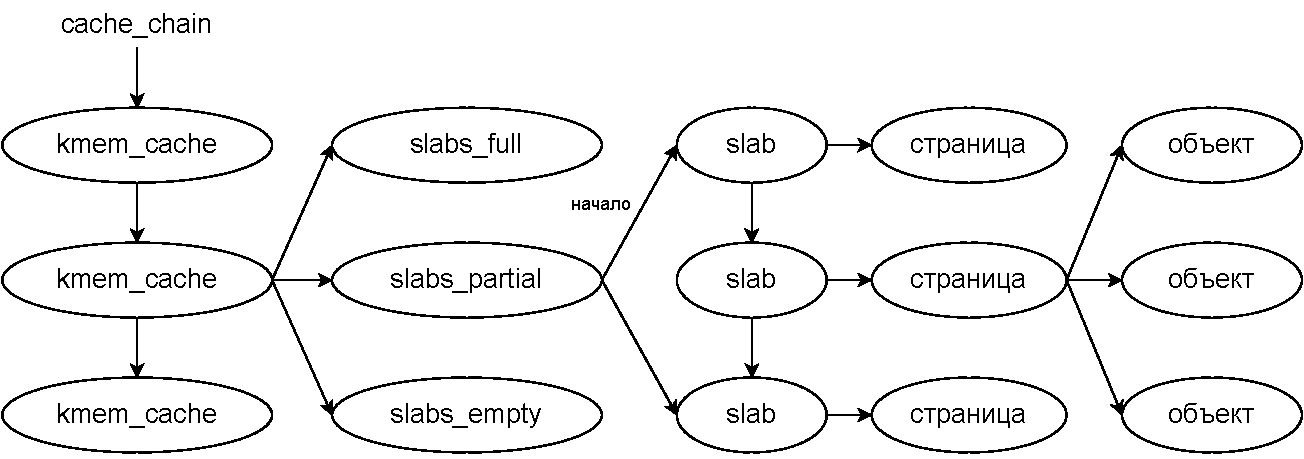
\includegraphics[width=0.8\linewidth]{./images/slabs.pdf}
	\end{tabular}
\end{table}

Каждый кеш содержит список слабов

Существует 3 слаба:
\begin{enumerate}
	\item slabs\_full -- заполненный
	\item slabs\_partial -- частично заполненный
	\item slabs\_empty -- пустой
\end{enumerate}

Объекты -- основные элементы, которые выделяются из спец. кеша и в него же возвращаются

slabs\_empty -- основные кандидаты на повторное использование

В случае распределения SLAB участки памяти, подходящие под размещение объектов данных определенного типа, определены заранее. Аллокатор SLAB (распределитель) хранит информацию о размещении этих участков, к-ые также известны как кеш

В результате, если поступает зпрос на выделение памяти для объекта определенного типа (скорее именно размера), то он удовлетворяется с помощью SLAB

\section{Функции для работы с кэшем SLAB. Примеры из лабораторной работы}
\begin{lstlisting}
	#define SLAB_NAME "my_vfs_cache"
	
	static struct kmem_cache *cache = NULL;
	static void **cache_mem_area = NULL;
	
	static struct file_system_type my_vfs_type = {
		.owner = THIS_MODULE,
		.name = "myvfs",
		.mount = my_vfs_mount,
		.kill_sb = my_kill_super,
	};
	
	static void func_init(void *p)
	{
		*(int *)p = (int)p;
	}
	
	static int __init my_vfs_init(void){
		int rc = register_filesystem(&my_vfs_type);
		// error handling
		if ((cache_mem_area = kmalloc(sizeof(void*), GFP_KERNEL)) == NULL)
		// error handling
		if ((cache = kmem_cache_create(SLAB_NAME, sizeof(my_vfs_inode), 0, SLAB_HWCACHE_ALIGN, func_init)) == NULL)
		// error handling
		if (((*cache_mem_area) = kmem_cache_alloc(cache, GFP_KERNEL)) == NULL)
		// ...
		return 0;
	}
	
	static void __exit my_vfs_exit(void)
	{
		kmem_cache_free(cache, *cache_mem_area);
		kmem_cache_destroy(cache);
		kfree(cache_mem_area);
		int rc = unregister_filesystem(&my_vfs_type);
		// ...
	}
	
	module_init(my_vfs_init);
	module_exit(my_vfs_exit);
\end{lstlisting}


\section{Функции, определенные на файлах\\
(struct file\_operations), функции, определенные на файлах, и их регистрация}
\subsection{Определение struct file\_operations}
\begin{lstlisting}
	struct file_operations {
		struct module *owner;
		loff_t (*llseek) (struct file *, loff_t, int);
		ssize_t (*read) (struct file *, char __user *, size_t, loff_t *);
		ssize_t (*write) (struct file *, const char __user *, size_t, loff_t *);
		...
		int (*open) (struct inode *, struct file *);
		...
		int (*release) (struct inode *, struct file *);
		...
	};
\end{lstlisting}

\subsection{Регистрация функций для работы с файлами}
Разработчики драйверов должны регистрировать свои функции read/write.

В Unix/linux все файл, чтобы все действия свести к однотипным операциям (read/write) и не ``размножать`` эти действия, а свести к небольшому набору операций.

Для регистрации своих функций read/write в драйверах используется struct file\_operations

С некоторой версии ядра появилась struct proc\_ops. В загружаемых модулях ядра можно использовать условную компиляцию
\begin{lstlisting}
	#if LINUX_VERSION_CODE >= KERNEL_VERSION(5,6,0)
	#define HAVE_PROC_OPS
	#endif
	#ifdef HAVE_PROC_OPS
	static struct proc_ops fops = {
		.proc_read = fortune_read,
		.proc_write = fortune_write,
		.proc_open = fortune_open,
		.proc_release = fortune_release,
	};
	#else
	static struct file_operations fops = {
		.owner = THIS_MODULE,
		.read = fortune_read,
		.write = fortune_write,
		.open = fortune_open,
		.release = fortune_release,
	};
	#endif
	\end{lstlisting}
	
	proc\_open и open имеют одни и те же формальные параметры (указатели на struct inode и на struct file)
	
	С остальными функциями аналогично. struct proc\_ops сделана, чтобы не вешаться на функции struct file\_operations, которые используются драйверами. Функции struct file\_operations настолько важны для работы системы, что их решили освободить от работы с ф.с. proc 
	
	\section{Пример из лабораторной работы по файловой системе /proc}
	\begin{lstlisting}
	#if LINUX_VERSION_CODE >= KERNEL_VERSION(5,16,0)
	#define HAVE_PROC_OPS
	#endif
	
	#define MAX_COOKIE_BUF_SIZE PAGE_SIZE
	
	static ssize_t fortune_write(struct file *file, const char __user *buf, size_t len, loff_t *ppos) 
	{
		// ...
		if (copy_from_user(&cookie_buffer[write_index], buf, len) != 0)
		// error handling
		write_index += len;
		cookie_buffer[write_index - 1] = '\0';
		return len;
	}
	
	static ssize_t fortune_read(struct file *file, char __user *buf, size_t len, loff_t *f_pos) 
	{
		// ...
		int read_len = snprintf(tmp_buffer, MAX_COOKIE_BUF_SIZE, "%s\n", &cookie_buffer[read_index]);
		if (copy_to_user(buf, tmp_buffer, read_len) != 0)
		// error handling
		read_index += read_len;
		*f_pos += read_len;
		return read_len;
	}
	
	#ifdef HAVE_PROC_OPS
	static struct proc_ops fops = {
		.proc_read = fortune_read,
		.proc_write = fortune_write,
		.proc_open = fortune_open,
		.proc_release = fortune_release,
	};
	#else
	static struct file_operations fops = {
		.owner = THIS_MODULE,
		.read = fortune_read,
		.write = fortune_write,
		.open = fortune_open,
		.release = fortune_release,
	};
	#endif
	
	static int __init fortune_init(void) 
	{
		if ((cookie_buffer = vzalloc(MAX_COOKIE_BUF_SIZE)) == NULL)
		// error handling
		if ((fortune_dir = proc_mkdir(FORTUNE_DIRNAME, NULL)) == NULL)
		// error handling
		if ((fortune_file = proc_create(FORTUNE_FILENAME, S_IRUGO | S_IWUGO, fortune_dir, &fops)) == NULL) 
		// error handling
		if ((fortune_symlink = proc_symlink(FORTUNE_SYMLINK, NULL, FORTUNE_PATH)) == NULL)
		// error handling
		printk(KERN_INFO " + module is loaded.\n");
		return 0;
	}
	
	static void __exit fortune_exit(void) 
	{
		// cleanup
		printk(KERN_INFO " + module is unloaded.\n");
	}
	
	module_init(fortune_init);
	module_exit(fortune_exit);
	\end{lstlisting}
	
	
